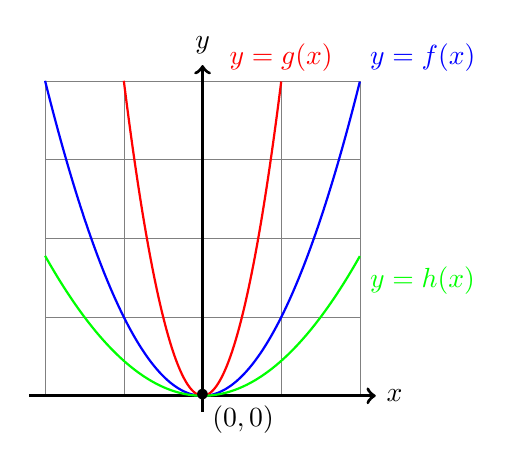
\begin{tikzpicture}
  \draw[very thin,color=gray] (-2,0) grid (2,4);

  \draw[very thick,->] (-2.2,0) -- (2.2,0) node[right] {$x$};
  \draw[very thick,->] (0,-.2) -- (0,4.2) node[above] {$y$};
  
  \draw [color=blue,thick] plot[smooth,samples=500,domain=-2:2] (\x,{(\x)^2}) node [above right] {$y = f(x)$};
  \draw [color=red,thick] plot[smooth,samples=500,domain=-1:1] (\x,{(2*\x)^2}) node [above] {$y = g(x)$};
  \draw [color=green,thick] plot[smooth,samples=500,domain=-2:2] (\x,{(2/3*\x)^2}) node [below right] {$y = h(x)$};

  \node at (0,0) {$\bullet$};
  \node [below right] at (0,0) {$(0,0)$};
\end{tikzpicture}
